\documentclass[border=4pt]{standalone}
\usepackage{fontspec}
\usepackage{amsmath}
\usepackage{unicode-math}
\setmainfont{Latin Modern Roman}
\setmathfont{Latin Modern Math}
\usepackage{pgfplots}
\usepackage{pgfplotstable}
\pgfplotsset{compat=1.18}
\usepackage{tkz-euclide}
\usetikzlibrary{arrows.meta,calc,angles,quotes,patterns,3d,backgrounds}
\definecolor{ink}{HTML}{123428}
\definecolor{asy}{HTML}{475569}
\definecolor{mint}{HTML}{86e0bd}
\tikzset{asym/.style={asy, line width=0.9pt, dash pattern=on 5pt off 3.5pt},
         guide/.style={gray!70, line width=0.6pt, densely dotted},
         dot/.style={circle, inner sep=0pt, minimum size=5pt, draw=white, line width=0.5pt},
         odot/.style={circle, inner sep=0pt, minimum size=5.5pt, fill=white, line width=1pt},
         lab/.style={font=\footnotesize, inner sep=1.5pt, text=ink}}
\begin{document}
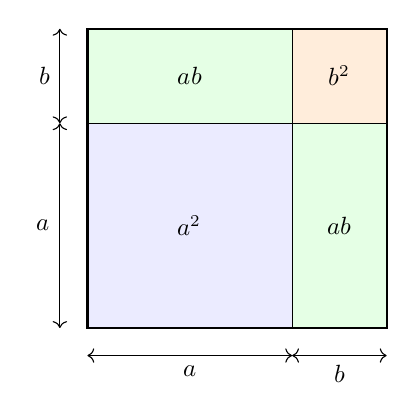
\begin{tikzpicture}[x=1cm,y=1cm,font=\small]
\fill[blue!8] (0,0) rectangle (2.6,2.6); \fill[green!10] (2.6,0) rectangle (3.8,2.6); \fill[green!10] (0,2.6) rectangle (2.6,3.8); \fill[orange!14] (2.6,2.6) rectangle (3.8,3.8);
\draw[thick] (0,0) rectangle (3.8,3.8); \draw (2.6,0)--(2.6,3.8); \draw (0,2.6)--(3.8,2.6);
\node at (1.3,1.3) {$a^2$}; \node at (3.2,1.3) {$ab$}; \node at (1.3,3.2) {$ab$}; \node at (3.2,3.2) {$b^2$};
\draw[<->] (0,-0.35)--(2.6,-0.35) node[midway,below] {$a$}; \draw[<->] (2.6,-0.35)--(3.8,-0.35) node[midway,below] {$b$};
\draw[<->] (-0.35,0)--(-0.35,2.6) node[midway,left] {$a$}; \draw[<->] (-0.35,2.6)--(-0.35,3.8) node[midway,left] {$b$};
\end{tikzpicture}
\end{document}
